\chapter{软件设计与分析}

\section{软件架构设计}

农业果实称重云端软件的架构设计采用分层的设计思想,将系统抽象为展示层、通信层、服务层和数据层。如图\ref{fig:软件分层架构图}所示。

\begin{figure}[H]
    \centering
    \includegraphics[width=0.8\linewidth]{../design/out/软件分层架构图.png}
    \caption{软件分层架构图}
    \label{fig:软件分层架构图}
\end{figure}

展示层包含了电子秤终端和网页端两个部分。其中电子秤终端是果实称重功能的具体表现,本系统将提供一个电子秤终端的模拟软件,来实现对称重流程的模拟。网页端则用于农场的信息管理和可视化,包括员工、电子秤、果实和采摘作业等。

通信层包含各类可以和系统进行通信的协议。展示层通过通信层所提供的协议和其它规则来完成和后台服务的数据通信。其中对于电子秤称重数据的提交,可以通过 HTTP/HTTPS、MQTT、CoAP、STOMP 等多种物联网通信协议来完成,其它信息管理和可视化相关接口则只支持 HTTP/HTTPS 协议。

服务层包含六个模块,用于实现具体的业务。各个模块等功能描述如下:

1、用户管理模块:实现农场用户的认证、信息管理、可视化相关功能。
2、果实模块:实现农场果实的信息管理、可视化相关功能。
3、工作服务模块:实现采摘作业的信息管理、可视化相关功能。
4、称重服务模块:实现电子秤的信息管理、称重数据的处理及可视化相关功能。
5、MQTT 服务模块:即 MQTT Broker,作为 MQTT 生产者和消费者的通信桥梁。
6、EMQX 服务模块:EMQX 提供了物联网网关功能,可以接收 CoAP、STOMP 等通信协议等消息,将其转换为 MQTT 消息与 MQTT Broker 通信。

数据层包含三个模块,MySQL 用于数据的持久化存储和迁移;Redis 作为一个缓存组件,存储一些读多写少的数据,以提高数据获取性能;MQTT 用于存储 MQTT 消息,主要服务于电子秤称重功能。

\section{服务接口设计}

本系统服务接口包含四个部分,分别是用户管理模块、果实模块、工作服务模块和称重服务模块。具体接口功能和路径设计如表格\ref{tab:用户管理模块接口设计}、表格\ref{tab:果实模块接口设计}、表格\ref{tab:工作服务模块接口设计}和表格\ref{tab:工作服务模块接口设计}所示。

% 用户管理模块表格
\begin{table}[H]
\centering
% \resizebox{\textwidth}{!}{%
\begin{tabular}{|c|c|c|}
\hline
\textbf{接口名称} & \textbf{HTTP方法} & \textbf{接口路径} \\
\hline
用户登录 & POST & /user/login \\
\hline
获取个人信息 & GET & /user \\
\hline
更新个人信息 & PUT & /user/me \\
\hline
获取用户列表 & GET & /user/list \\
\hline
获取用户信息 & GET & /user/{uid} \\
\hline
添加用户 & POST & /user \\
\hline
更新用户 & PUT & /user \\
\hline
\end{tabular}%

    % }
\caption{用户管理模块接口设计}
\label{tab:用户管理模块接口设计}
\end{table}

% 果实模块表格
\begin{table}[H]
\centering
% \resizebox{\textwidth}{!}{%
\begin{tabular}{|c|c|c|}
\hline
\textbf{接口名称} & \textbf{HTTP方法} & \textbf{接口路径} \\
\hline
获取果实列表 & GET & /produce/list \\
\hline
获取果实 & GET & /produce/{id} \\
\hline
根据名称获取果实 & GET & /produce \\
\hline
添加果实 & POST & /produce \\
\hline
更新果实 & PUT & /produce \\
\hline
获取果实年产量 & GET & /produce/summary/year \\
\hline
获取果实分批产量 & GET & /produce/summary/work \\
\hline
\end{tabular}%

% }
\caption{果实模块接口设计}
\label{tab:果实模块接口设计}
\end{table}

% 工作服务模块表格
\begin{table}[H]
\centering
% \resizebox{\textwidth}{!}{%
\begin{tabular}{|c|c|c|}
\hline
\textbf{接口名称} & \textbf{HTTP方法} & \textbf{接口路径} \\
\hline
获取采摘工作列表 & GET & /work/list \\
\hline
获取采摘工作 & GET & /work/{id} \\
\hline
获取果实的采摘工作列表 & GET & /work/produce/{id} \\
\hline
添加采摘工作 & POST & /work \\
\hline
更新采摘工作 & PUT & /work \\
\hline
获取采摘作业的分配情况 & GET & /work/{id}/assignments \\
\hline
获取我被分配的工作 & GET & /work/assignments/me \\
\hline
分配工作 & POST & /work/assign \\
\hline
重新分配工作 & PUT & /work/assign \\
\hline
\end{tabular}%

% }
\caption{工作服务模块接口设计}
\label{tab:工作服务模块接口设计}
\end{table}

% 称重服务模块表格
\begin{table}[H]
\centering
% \resizebox{\textwidth}{!}{%
\begin{tabular}{|c|c|c|}
\hline
\textbf{接口名称} & \textbf{HTTP方法} & \textbf{接口路径} \\
\hline
获取电子秤列表 & GET & /weigh/scale/list \\
\hline
获取电子秤 & GET & /weigh/scale/{id} \\
\hline
根据key获取电子秤 & GET & /weigh/scale \\
\hline
添加电子秤 & POST & /weigh/scale \\
\hline
更新电子秤信息 & PUT & /weigh/scale \\
\hline
添加称重记录 & POST & /weigh/record \\
\hline
获取称重记录 & POST & /weigh/record/list \\
\hline
获取员工各作业采摘量 & GET & /weigh/summary \\
\hline
\end{tabular}%

% }
\caption{称重服务模块接口设计}
\label{tab:称重服务模块接口设计}
\end{table}

\section{关键功能设计}

\section{通信流程设计}

市面上的电子秤支持多种通信协议。对于支持 TCP/IP 的物联网设备,可以通过 WIFI、蜂窝网络以及以太网,使用 HTTP、MQTT、CoAP、LwM2M 以及 XMPP 等应用层协议协议接入云端。

\begin{figure}[H]
    \centering
    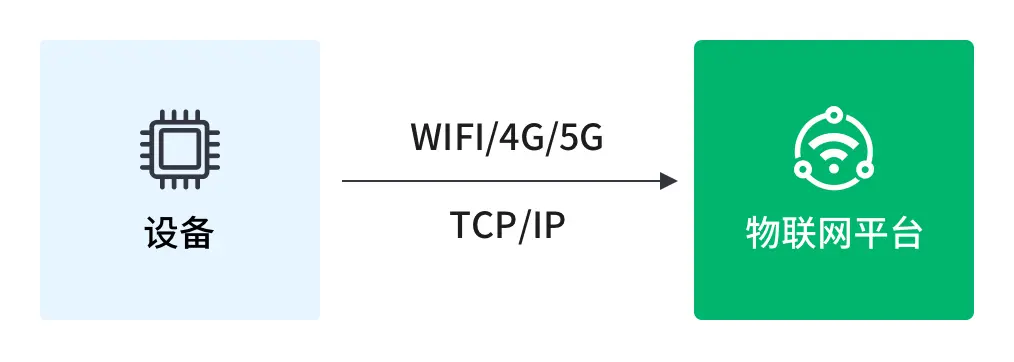
\includegraphics[width=0.8\linewidth]{../design/IoT1.png}
    \caption{IoT1}
    \label{fig:IoT1}
\end{figure}

网关协议是适用于短距通信无法直接上云的协议,比如蓝牙、ZigBee、LoRa 等。此类设备需要接入网关转换之后,通过 TCP/IP 协议进行上云。

\begin{figure}[H]
    \centering
    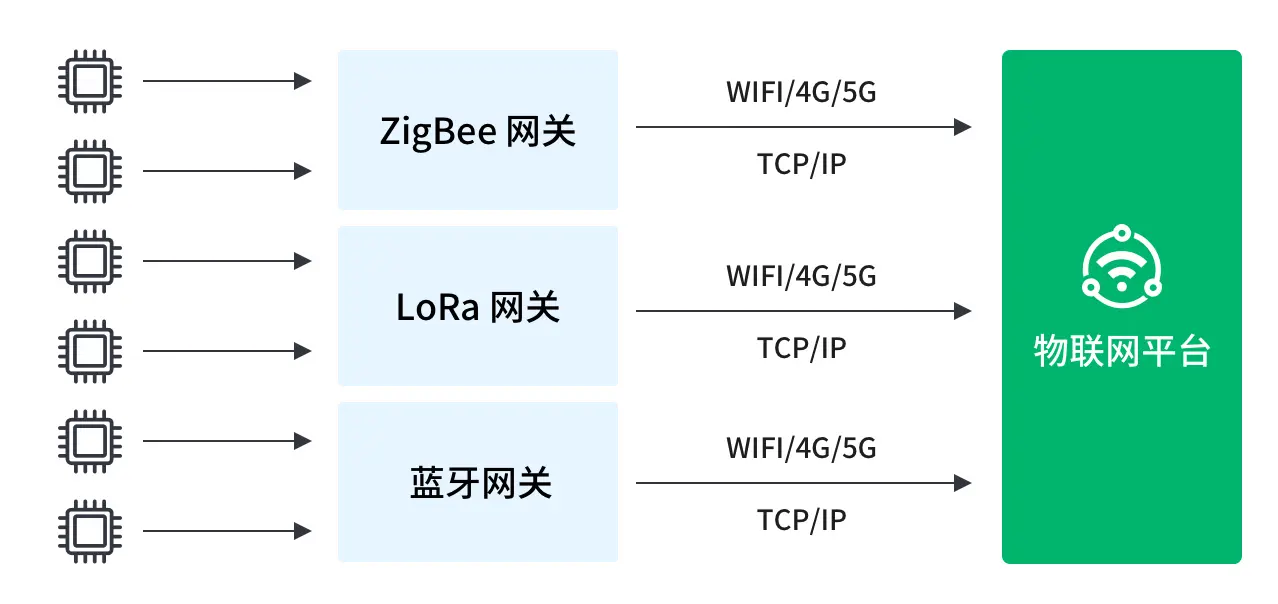
\includegraphics[width=0.8\linewidth]{../design/IoT2.png}
    \caption{IoT2}
    \label{fig:IoT2}
\end{figure}

本系统不考虑网关协议,只考虑应用层协议。系统将支持不同种类的电子秤,支持包含 HTTP、MQTT、MQTT-SN、CoAP、STOMP 在内的多种物联网通信协议。

为了降低开发成本,除了 HTTP、MQTT 这两种通信协议,其它物联网协议采用网关转换的方法来提供支持,网关将对各类协议转换成 MQTT 协议与 MQTT Broker 进行通信,认证规则和消息的持久化规则遵循 MQTT 协议标准。

这里主要分析两种协议:HTTP 和 MQTT。

HTTP(HyperText Transfer Protocol)即超文本传输协议,是一种用于分布式、协作式和超媒体信息系统的应用层协议。在电子秤系统中,通过调用 HTTP 接口上传称重信息具有以下特点:

一、稳定性和通用性:HTTP 是互联网上广泛使用的协议,具有很高的稳定性和通用性。几乎所有的网络设备和软件都支持 HTTP 协议,这使得电子秤可以很容易地与各种不同的系统进行集成。无论是传统的服务器架构,还是现代的云服务平台,都可以通过 HTTP 接口接收电子秤上传的称重信息。例如,许多企业的内部管理系统、电商平台的库存管理系统等都可以通过 HTTP 接口与电子秤进行数据交互,实现实时的库存更新和物流跟踪\cite{Zhao2016}。

二、易于开发和调试:HTTP 协议的开发和调试工具非常丰富。开发人员可以使用常见的编程语言和开发框架,如 Java、Python、Node.js 等,轻松地实现 HTTP 接口的调用和数据处理。同时,各种网络调试工具,如 Postman、Fiddler 等,可以帮助开发人员快速地测试和调试电子秤与服务器之间的通信,确保数据的准确传输。

三、支持多种数据格式:HTTP 协议支持多种数据格式的传输,如 JSON、XML 等。这使得电子秤可以根据不同的应用需求,选择合适的数据格式上传称重信息。例如,对于需要与第三方系统进行数据集成的场景,可以选择使用 JSON 格式,因为 JSON 格式具有简洁、易读、易于解析等优点,被广泛应用于 Web 开发和数据交换领域。

MQTT(Message Queuing Telemetry Transport)即消息队列遥测传输协议,是一种轻量级的发布/订阅模式的消息传输协议。在电子秤系统中,发送 MQTT 消息上传称重信息具有以下优势:

一、低带宽和低功耗:MQTT 协议非常适合在低带宽和低功耗的环境下使用。对于电子秤等物联网设备来说,通常需要在有限的网络资源和电池电量下进行数据传输。MQTT 协议通过采用轻量级的消息格式和高效的发布/订阅模式,可以大大降低网络带宽的占用和设备的功耗。例如,在一些偏远地区或者移动环境下,网络带宽可能非常有限,此时使用 MQTT 协议可以确保电子秤能够及时上传称重信息,同时不会对网络造成过大的负担\cite{Jia2015}。

二、实时性和可靠性:MQTT 协议支持 QoS(Quality of Service)级别,可以根据不同的应用需求,选择不同的消息传输质量级别。在 MQTT 协议中,QoS 有三种级别\cite{Jia2015},分别是:

1、QoS0 – “最多一次”:消息最多传送一次,不保证消息到达目标。适用于实时性要求非常高,但对消息丢失容忍的场景。

2、QoS1 – “至少一次”:保证消息至少传送一次,但可能会重复。适用于需要消息可靠到达,但不介意重复接收的情况。

3、QoS2 – “只有一次”:确保每条消息只会传送一次,且无重复。适用于对消息的唯一性和可靠性有较高要求的场景。

对于需要实时上传称重信息的场景,可以选择 QoS1 或 QoS2 级别,确保消息的可靠传输。同时,MQTT 协议的发布/订阅模式可以实现实时的数据推送,当电子秤上传称重信息后,订阅了该主题的客户端可以立即收到消息,实现实时的数据更新。

三、易于扩展和集成:MQTT 协议具有良好的扩展性和集成性。可以很容易地与其他物联网协议和技术进行集成,如 CoAP、HTTP、WebSocket 等。同时,MQTT 协议的发布/订阅模式可以支持大规模的设备连接和数据传输,适用于构建物联网应用平台。例如,在智慧农业大棚测控系统中,采用 MQTT 协议将智慧大棚测控系统和阿里云物联网平台结合在一起,通过手机 APP 或 PC 软件访问阿里云服务器数据库,实现了移动终端对农业大棚实时监测和控制\cite{Liang2020}。

\section{数据库设计}

本软件数据库设计分为三个阶段:概念模型设计、逻辑模型设计和物理模型设计,下面进行具体阐述。

\subsection{概念模型设计}

农业果实称重云端软件中,可以抽象出七个实体对象,分别是果实、员工、电子秤、采摘作业、称重记录、MQTT客户端、MQTT授权信息,具体分析如下:

1、果实(Fruit):代表农场中的果实,具有编号(ID)属性。

2、员工(Employee):代表农场中的员工,具有编号(ID)属性。

3、电子秤(Electronic Scale):代表用于称重果实的电子秤,具有编号(ID)和密钥(Key)属性。

4、MQTT 客户端(MQTT Client):代表用于连接 MQTT 服务器的客户端,具有编号(ID)和密码(Password)属性。

5、采摘作业(Picking Task):代表员工采摘果实的作业,具有开始时间、结束时间和采摘结果属性。

6、称重记录(Weighing Record):代表电子秤记录的果实重量,具有称重结果和称重时间属性。

7、MQTT 授权信息(MQTT Authorization Info):代表 MQTT 客户端的授权信息,具有权限信息属性。

针对上述对象,根据实际的业务场景,可以得到如下关系:

\begin{table}[H]
\centering
\resizebox{\textwidth}{!}{%
\begin{tabular}{|c|c|c|}
\hline
\textbf{关系名称} & \textbf{关系类型} & \textbf{描述} \\
\hline
果实 - 采摘关系 & 一对多(1:N) & 一个果实可以被多次采摘,与多个采摘作业相关联。 \\
\hline
员工 - 员工称重记录 & 一对多(1:N) & 一个员工可以进行多次称重记录。  \\
\hline
员工 - 采摘作业 & 一对多(1:N) & 一个员工可以执行多个采摘作业。  \\
\hline
电子秤 - 电子秤称重记录 & 一对多(1:N) & 一个电子秤可以记录多个称重记录。  \\
\hline
电子秤 - 称重记录 & 一对多(1:N) & 一个电子秤可以记录多个称重记录。\\
\hline
采摘作业 - 称重记录 & 一对多(1:N) & 一个采摘作业可以产生多个称重记录(例如,在不同时间多次称重)。  \\
\hline
MQTT 客户端 - 设备认证 & 一对一(1:1) & 每个 MQTT 客户端都必须进行设备认证。 \\
\hline
MQTT 客户端 - 设备授权 & 一对多(1:N) & 一个 MQTT 客户端可以拥有多个授权信息。  \\
\hline
员工 - 称重记录 & 一对多(1:N) & 一个员工可以产生多个称重记录。\\
\hline
电子秤 - 设备认证 & 一对一(1:1) & 每个电子秤都必须进行设备认证。  \\
\hline
\end{tabular}%
}
\caption{实体关系及属性表}
\end{table}

将上述分析进行归纳,得到 ER 图如下:

\begin{figure}[H]
    \centering
    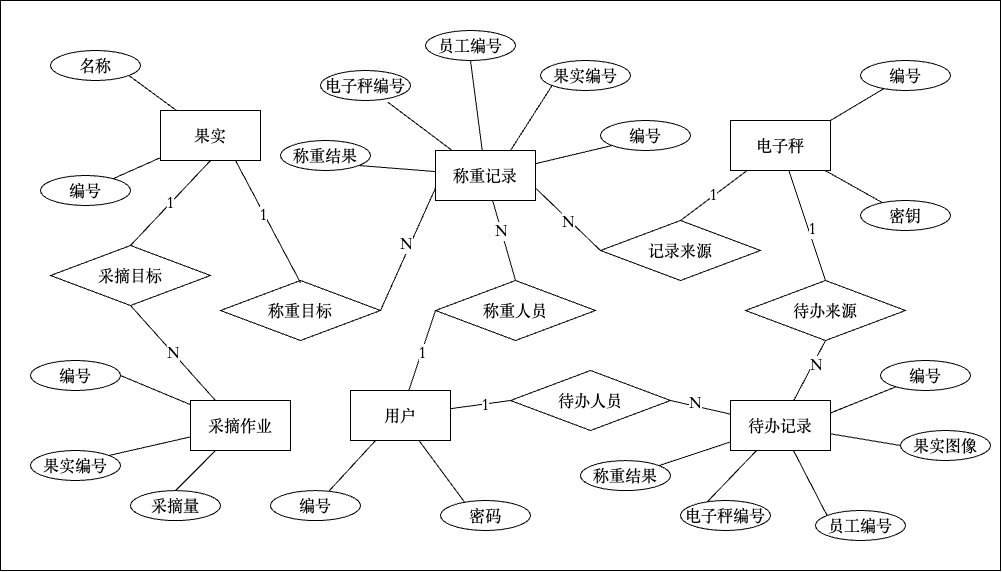
\includegraphics[width=0.8\linewidth]{../design/数据库概念模型设计.png}
    \caption{数据库概念模型设计}
    \label{fig:数据库概念模型设计}
\end{figure}

该 ER 图展示了一个农场管理系统中各个实体之间的复杂关系,包括果实、员工、电子秤和 MQTT 客户端。通过这些关系,系统可以有效地跟踪果实的采摘、称重和授权信息,从而实现高效的农场管理。

\subsection{逻辑模型设计}

本部分详细描述了系统各个表的结构及其字段定义,涵盖了表之间的关系、字段的数据类型及约束条件。每个表的设计都遵循规范化原则,以确保数据的一致性、完整性和高效性。字段的定义包括主键、外键、唯一约束、非空约束等,同时考虑了查询和更新的效率,力求在保证系统扩展性的同时,实现良好的性能表现。

% t_user
\begin{table}[H]
    \centering
    \caption{用户表 (t\_user)}
    \begin{tabular}{|l|l|l|l|}
    \hline
    字段 & 类型 & 约束 & 说明 \\
    \hline
    id & bigint & 主键 & 自增主键 \\
    uid & varchar(255) & 非空,唯一 & 用户认证编号 \\
    name & varchar(255) & 非空 & 用户名称 \\
    password & varchar(255) & 非空 & 密码(加密) \\
    roles & varchar(255) & - & 角色(英文逗号分隔) \\
    create\_time & bigint & 非空 & 创建时间(毫秒级时间戳) \\
    update\_time & bigint & 非空 & 更新时间(毫秒级时间戳) \\
    status & int & 非空 & 状态(0禁用/1启用/2已删除) \\
    \hline
    \end{tabular}
    \end{table}

% t_produce
\begin{table}[H]
\centering
\caption{果实表 (t\_produce)}
\begin{tabular}{|l|l|l|l|}
\hline
字段 & 类型 & 约束 & 说明 \\
\hline
id & bigint & 主键 & 系统自带从0开始,用户添加从1000000开始 \\
name & varchar(255) & 非空,唯一 & 果实名称 \\
name\_en & varchar(255) & 唯一 & 果实英文名称 \\
create\_time & bigint & 非空 & 创建时间(毫秒级时间戳) \\
update\_time & bigint & 非空 & 更新时间(毫秒级时间戳) \\
status & int & 非空 & 状态(0未种植/1在种植/2已删除) \\
\hline
\end{tabular}
\end{table}

% ## t_work
\begin{table}[H]
\centering
\caption{采摘作业表 (t\_work)}
\begin{tabular}{|l|l|l|l|}
\hline
字段 & 类型 & 约束 & 说明 \\
\hline
id & bigint & 主键 & 自增主键 \\
produce\_id & bigint & 非空 & 果实编号 \\
start\_time & bigint & 非空 & 采摘开始时间(毫秒级时间戳) \\
end\_time & bigint & 非空 & 采摘结束时间(毫秒级时间戳) \\
data\_value & decimal(10,2) & - & 总的采摘称重结果 \\
unit & int & - & 称重单位(0mg/1g/2kg/3t/4lb/5oz/6ct) \\
create\_time & bigint & 非空 & 创建时间(毫秒级时间戳) \\
update\_time & bigint & 非空 & 更新时间(毫秒级时间戳) \\
status & int & 非空 & 状态(0未开始/1进行中/2已结束/3已取消/4已删除) \\
\hline
\end{tabular}
\end{table}

% t_scale
\begin{table}[H]
\centering
\caption{电子秤表 (t\_scale)}
\begin{tabular}{|l|l|l|l|}
\hline
字段 & 类型 & 约束 & 说明 \\
\hline
id & bigint & 主键 & 自增主键 \\
sid & varchar(255) & 非空 & MQTT 用户认证编号 \\
model & varchar(255) & - & 型号 \\
max\_capacity & decimal(10,2) & 非空 & 最大量程 \\
min\_capacity & decimal(10,2) & 非空 & 最小量程 \\
unit & int & 非空 & 量程单位(0mg/1g/2kg/3t/4lb/5oz/6ct) \\
verification\_interval & int & - & 检定分度值 \\
display\_interval & int & - & 显示分度值 \\
unit\_dv & int & - & 分度值单位(0mg/1g/2kg/3t/4lb/5oz/6ct) \\
protocol & varchar(255) & - & 协议(小写,逗号分隔) \\
create\_time & bigint & 非空 & 创建时间(毫秒级时间戳) \\
update\_time & bigint & 非空 & 更新时间(毫秒级时间戳) \\
status & int & 非空 & 状态(0禁用/1启用/2已删除) \\
\hline
\end{tabular}
\end{table}

% t_record
\begin{table}[H]
\centering
\caption{称重记录表 (t\_record)}
\begin{tabular}{|l|l|l|l|}
\hline
字段 & 类型 & 约束 & 说明 \\
\hline
id & bigint & 主键 & 自增主键 \\
work\_id & bigint & 非空 & 采摘作业编号 \\
produce\_id & bigint & 非空 & 果实编号 \\
image & varchar(255) & - & 果实图片地址 \\
employee\_id & bigint & 非空 & 员工编号 \\
scale\_id & bigint & 非空 & 电子秤编号 \\
data\_value & decimal(10,2) & 非空 & 称重结果 \\
data\_error\_margin & decimal(10,2) & - & 称量结果误差范围 \\
unit & int & 非空 & 称重单位(0mg/1g/2kg/3t/4lb/5oz/6ct) \\
data\_time & bigint & 非空 & 称重时间(毫秒级时间戳) \\
\hline
\end{tabular}
\end{table}

% t_todo
\begin{table}[H]
\centering
\caption{待处理称重记录表 (t\_todo)}
\begin{tabular}{|l|l|l|l|}
\hline
字段 & 类型 & 约束 & 说明 \\
\hline
id & bigint & 主键 & 自增主键 \\
produce\_id & bigint & - & 果实编号 \\
produce\_name & varchar(255) & - & 果实名称 \\
image & varchar(255) & - & 采摘作业图片地址 \\
employee\_id & bigint & 非空 & 员工编号 \\
scale\_id & bigint & 非空 & 电子秤编号 \\
data\_value & decimal(10,2) & 非空 & 称重结果 \\
data\_error\_margin & decimal(10,2) & - & 称量结果误差范围 \\
unit & int & 非空 & 称重单位(0mg/1g/2kg/3t/4lb/5oz/6ct) \\
data\_time & bigint & 非空 & 称重时间(毫秒级时间戳) \\
\hline
\end{tabular}
\end{table}

% ## t_mqtt_acl
\begin{table}[H]
\centering
\caption{MQTT 访问控制表 (t\_mqtt\_acl)}
\begin{tabular}{|l|l|l|l|}
\hline
字段 & 类型 & 约束 & 说明 \\
\hline
id & int & 主键 & 自增主键 \\
username & varchar(255) & 非空 & MQTT 认证用户名 \\
permission & varchar(255) & 非空 & 操作权限(allow/deny,即允许/拒绝) \\
action & varchar(255) & 非空 & 操作类型(publish/subscribe/all,即发布/订阅/所有) \\
topic & varchar(255) & 非空 & 适用主题 \\
qos & int & - & 消息 QoS 级别(0,1,2) \\
retain & int & - & 是否支持发布保留消息(0否/1是) \\
\hline
\end{tabular}
\end{table}

\subsection{物理模型设计}

本系统使用 MySQL 作为数据库管理系统,采用 InnoDB 存储引擎,事务隔离级别设置为可重复读,以确保数据的一致性和可靠性。在后台应用中,数据库访问通过 JPA (Java Persistence API) 进行实现,简化了数据库操作,提升了代码的可维护性和开发效率。

\section{本章小结}

这些设计模式和架构描述展示了农业果实称重云端软件系统的整体设计和通信流程。通过采用前后端分离的架构,结合 Spring 后端的 MVC 模式与 Vue 前端的 MVVM 模式,系统能够更好地处理数据交互和界面更新。系统架构通过分层设计,使得每一层都具备明确的职责,方便后期的扩展和维护。

在通信协议部分,系统的选择了 HTTP 和 MQTT 两种协议,分别适用于不同的应用场景。HTTP 用于传统的接口交互,而 MQTT 则通过低带宽、高可靠性和实时性的优势,适应了物联网环境中的需求。这两种协议的结合使得系统可以灵活应对不同类型的设备和网络条件。

数据库设计部分,构建了清晰的实体关系,确保了数据的完整性和系统的高效运行。通过一对多的关系设计,系统能够记录和管理员工、电子秤、果实等多个维度的数据,从而支持各种业务场景。
